\newpage
\section{Euclid's Proof of Someone's Theorem}

\begin{prob}
Remind us, what is the most famous theorem of all and what exactly
does it assert?
\end{prob}

\begin{prob} 
What would one need to prove about the following diagram to prove the
``most famous theorem of all?''
\[
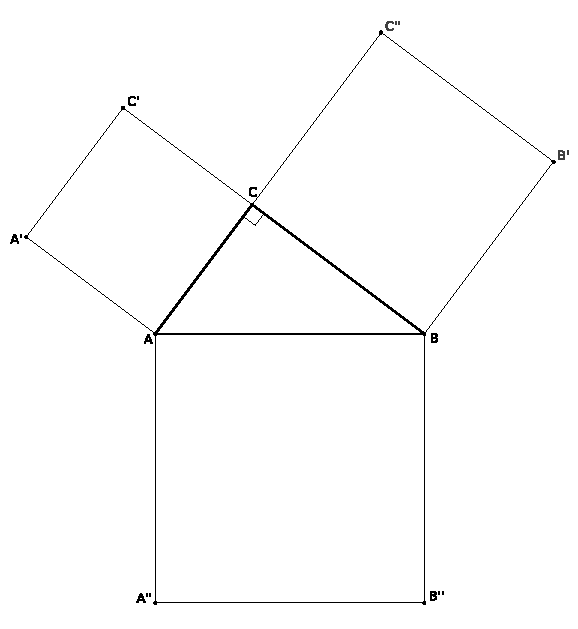
\includegraphics{../graphics/PythEuclid.pdf}
\]
\end{prob}

Let's see if we can do this!


\begin{prob}
Draw a line perpendicular to $\bar{AB}$ that passes though both $C$
and $\bar{A'' B''}$. Call the intersection between this line and
$\bar{AB}$, point $E$; call the intersection point between this line
and $\bar{A''B''}$, point $E'$. Explain why $\tri ACA''$ has half the
area of rectangle $AEE'A''$.
\end{prob}

\begin{prob}
Explain why $\tri ABA'$ has half the area of square $ACC'A'$.
\end{prob}

\begin{prob}
Explain why $\tri ACA''$ is congruent to $\tri ABA'$. 
\end{prob}

\begin{prob}
Explain why area of square $ACC'A'$ is equal to the area of rectangle
$AEE'A''$.
\end{prob}


\begin{prob}
Use similar ideas to complete a proof the ``most famous theorem of
all.''
\end{prob}


